\section{moeo\-Contribution\-Metric$<$ Objective\-Vector $>$ Class Template Reference}
\label{classmoeoContributionMetric}\index{moeoContributionMetric@{moeoContributionMetric}}
The contribution metric evaluates the proportion of non-dominated solutions given by a Pareto set relatively to another Pareto set (Meunier, Talbi, Reininger: 'A multiobjective genetic algorithm for radio network optimization', in Proc.  


{\tt \#include $<$moeo\-Contribution\-Metric.h$>$}

Inheritance diagram for moeo\-Contribution\-Metric$<$ Objective\-Vector $>$::\begin{figure}[H]
\begin{center}
\leavevmode
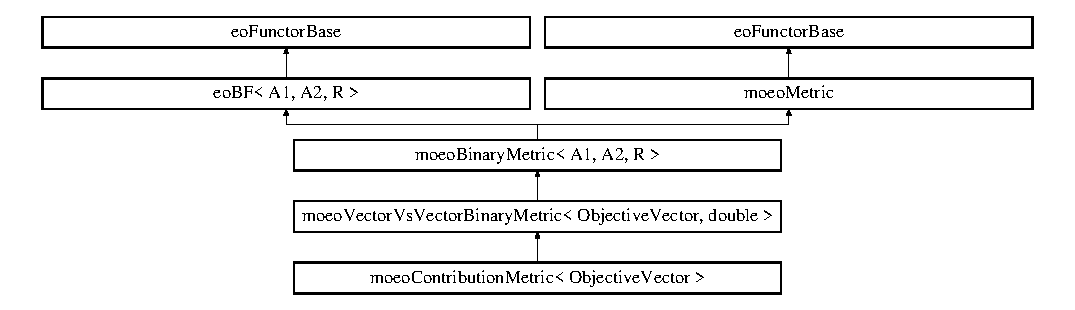
\includegraphics[height=3.71353cm]{classmoeoContributionMetric}
\end{center}
\end{figure}
\subsection*{Public Member Functions}
\begin{CompactItemize}
\item 
double \bf{operator()} (const std::vector$<$ Objective\-Vector $>$ \&\_\-set1, const std::vector$<$ Objective\-Vector $>$ \&\_\-set2)
\begin{CompactList}\small\item\em Returns the contribution of the Pareto set '\_\-set1' relatively to the Pareto set '\_\-set2'. \item\end{CompactList}\end{CompactItemize}
\subsection*{Private Member Functions}
\begin{CompactItemize}
\item 
unsigned int \bf{card\_\-C} (const std::vector$<$ Objective\-Vector $>$ \&\_\-set1, const std::vector$<$ Objective\-Vector $>$ \&\_\-set2)
\begin{CompactList}\small\item\em Returns the number of solutions both in '\_\-set1' and '\_\-set2'. \item\end{CompactList}\item 
unsigned int \bf{card\_\-W} (const std::vector$<$ Objective\-Vector $>$ \&\_\-set1, const std::vector$<$ Objective\-Vector $>$ \&\_\-set2)
\begin{CompactList}\small\item\em Returns the number of solutions in '\_\-set1' dominating at least one solution of '\_\-set2'. \item\end{CompactList}\item 
unsigned int \bf{card\_\-N} (const std::vector$<$ Objective\-Vector $>$ \&\_\-set1, const std::vector$<$ Objective\-Vector $>$ \&\_\-set2)
\begin{CompactList}\small\item\em Returns the number of solutions in '\_\-set1' having no relation of dominance with those from '\_\-set2'. \item\end{CompactList}\end{CompactItemize}
\subsection*{Private Attributes}
\begin{CompactItemize}
\item 
\bf{moeo\-Pareto\-Objective\-Vector\-Comparator}$<$ Objective\-Vector $>$ \bf{pareto\-Comparator}\label{classmoeoContributionMetric_b474229c85ffbf5108f51eef01ab2d64}

\begin{CompactList}\small\item\em Functor to compare two objective vectors according to Pareto dominance relation. \item\end{CompactList}\end{CompactItemize}


\subsection{Detailed Description}
\subsubsection*{template$<$class Objective\-Vector$>$ class moeo\-Contribution\-Metric$<$ Objective\-Vector $>$}

The contribution metric evaluates the proportion of non-dominated solutions given by a Pareto set relatively to another Pareto set (Meunier, Talbi, Reininger: 'A multiobjective genetic algorithm for radio network optimization', in Proc. 

of the 2000 Congress on Evolutionary Computation, IEEE Press, pp. 317-324) 



Definition at line 24 of file moeo\-Contribution\-Metric.h.

\subsection{Member Function Documentation}
\index{moeoContributionMetric@{moeo\-Contribution\-Metric}!operator()@{operator()}}
\index{operator()@{operator()}!moeoContributionMetric@{moeo\-Contribution\-Metric}}
\subsubsection{\setlength{\rightskip}{0pt plus 5cm}template$<$class Objective\-Vector$>$ double \bf{moeo\-Contribution\-Metric}$<$ Objective\-Vector $>$::operator() (const std::vector$<$ Objective\-Vector $>$ \& {\em \_\-set1}, const std::vector$<$ Objective\-Vector $>$ \& {\em \_\-set2})\hspace{0.3cm}{\tt  [inline]}}\label{classmoeoContributionMetric_491610f6557874c2989eaa7a75117dcb}


Returns the contribution of the Pareto set '\_\-set1' relatively to the Pareto set '\_\-set2'. 

\begin{Desc}
\item[Parameters:]
\begin{description}
\item[{\em \_\-set1}]the first Pareto set \item[{\em \_\-set2}]the second Pareto set \end{description}
\end{Desc}


Definition at line 33 of file moeo\-Contribution\-Metric.h.

References moeo\-Contribution\-Metric$<$ Objective\-Vector $>$::card\_\-C(), moeo\-Contribution\-Metric$<$ Objective\-Vector $>$::card\_\-N(), and moeo\-Contribution\-Metric$<$ Objective\-Vector $>$::card\_\-W().\index{moeoContributionMetric@{moeo\-Contribution\-Metric}!card_C@{card\_\-C}}
\index{card_C@{card\_\-C}!moeoContributionMetric@{moeo\-Contribution\-Metric}}
\subsubsection{\setlength{\rightskip}{0pt plus 5cm}template$<$class Objective\-Vector$>$ unsigned int \bf{moeo\-Contribution\-Metric}$<$ Objective\-Vector $>$::card\_\-C (const std::vector$<$ Objective\-Vector $>$ \& {\em \_\-set1}, const std::vector$<$ Objective\-Vector $>$ \& {\em \_\-set2})\hspace{0.3cm}{\tt  [inline, private]}}\label{classmoeoContributionMetric_4e60849763aaad0cdea66e71edf2d29e}


Returns the number of solutions both in '\_\-set1' and '\_\-set2'. 

\begin{Desc}
\item[Parameters:]
\begin{description}
\item[{\em \_\-set1}]the first Pareto set \item[{\em \_\-set2}]the second Pareto set \end{description}
\end{Desc}


Definition at line 54 of file moeo\-Contribution\-Metric.h.

Referenced by moeo\-Contribution\-Metric$<$ Objective\-Vector $>$::operator()().\index{moeoContributionMetric@{moeo\-Contribution\-Metric}!card_W@{card\_\-W}}
\index{card_W@{card\_\-W}!moeoContributionMetric@{moeo\-Contribution\-Metric}}
\subsubsection{\setlength{\rightskip}{0pt plus 5cm}template$<$class Objective\-Vector$>$ unsigned int \bf{moeo\-Contribution\-Metric}$<$ Objective\-Vector $>$::card\_\-W (const std::vector$<$ Objective\-Vector $>$ \& {\em \_\-set1}, const std::vector$<$ Objective\-Vector $>$ \& {\em \_\-set2})\hspace{0.3cm}{\tt  [inline, private]}}\label{classmoeoContributionMetric_68d6d1ec1ed0bed1ea290cdacb93b5b2}


Returns the number of solutions in '\_\-set1' dominating at least one solution of '\_\-set2'. 

\begin{Desc}
\item[Parameters:]
\begin{description}
\item[{\em \_\-set1}]the first Pareto set \item[{\em \_\-set2}]the second Pareto set \end{description}
\end{Desc}


Definition at line 71 of file moeo\-Contribution\-Metric.h.

References moeo\-Contribution\-Metric$<$ Objective\-Vector $>$::pareto\-Comparator.

Referenced by moeo\-Contribution\-Metric$<$ Objective\-Vector $>$::operator()().\index{moeoContributionMetric@{moeo\-Contribution\-Metric}!card_N@{card\_\-N}}
\index{card_N@{card\_\-N}!moeoContributionMetric@{moeo\-Contribution\-Metric}}
\subsubsection{\setlength{\rightskip}{0pt plus 5cm}template$<$class Objective\-Vector$>$ unsigned int \bf{moeo\-Contribution\-Metric}$<$ Objective\-Vector $>$::card\_\-N (const std::vector$<$ Objective\-Vector $>$ \& {\em \_\-set1}, const std::vector$<$ Objective\-Vector $>$ \& {\em \_\-set2})\hspace{0.3cm}{\tt  [inline, private]}}\label{classmoeoContributionMetric_df26b17120ed2271a6d1ec9c8c77b451}


Returns the number of solutions in '\_\-set1' having no relation of dominance with those from '\_\-set2'. 

\begin{Desc}
\item[Parameters:]
\begin{description}
\item[{\em \_\-set1}]the first Pareto set \item[{\em \_\-set2}]the second Pareto set \end{description}
\end{Desc}


Definition at line 89 of file moeo\-Contribution\-Metric.h.

References moeo\-Contribution\-Metric$<$ Objective\-Vector $>$::pareto\-Comparator.

Referenced by moeo\-Contribution\-Metric$<$ Objective\-Vector $>$::operator()().

The documentation for this class was generated from the following file:\begin{CompactItemize}
\item 
moeo\-Contribution\-Metric.h\end{CompactItemize}
